% Dèan sabaid an aghaidh bàs an t-solais!
% Infuria contro la morte del luce!
\documentclass{scrartcl}
%----------------------------------------------------------------------------------------
% Packages
\usepackage{graphicx} % Required for inserting images
% \usepackage{url}
\usepackage{xurl}
\usepackage{authblk}
\usepackage[hidelinks]{hyperref}
\usepackage[nomarkers]{endfloat}
\usepackage[toc,page]{appendix}
%----------------------------------------------------------------------------------------
\usepackage[
    backend=biber,
    style=authoryear
]{biblatex}
% \usepackage[
%     notes,
%     backend=biber,
%     % eprint=false,
%     % doi=false,
%     % related=false,
%     % url=false,    
% ]{biblatex-chicago}
%--------------------------------------------------------------------------------------
% \renewcommand{\cite}{\footcite} % For chicago notes style override the \cite command
\renewcommand{\cite}{\parencite}
% \renewcommand{\cite}{\autocite} 
%--------------------------------------------------------------------------------------
\addbibresource{main.bib}

%--------------------------------------------------------------------------------------
% Commands
\providecommand{\tightlist}{%
  \setlength{\itemsep}{0pt}\setlength{\parskip}{0pt}}

%----------------------------------------------------------------------------------------
% Title
\title{To See Oursels as Ithers See Us}
\subtitle{Updating the Melville Monument, Edinburgh 2016 - 2025}
\author[1]{Agnes Michalczyk}
\author[2]{Matthew Hamilton}
\affil[1]{Freie Universität Berlin / University of Edinburgh}
\affil[2]{Università di Bologna / University of Edinburgh}
\date{}
%----------------------------------------------------------------------------------------
% Main Article
\begin{document}

\maketitle

\begin{abstract}
The historical legacy by which Scotland was intertwined with England, formalised through the Acts of Union in 1707, has deeply shaped national narratives of the country's role within British colonialism and the transatlantic slave trade. Often presenting itself as the lesser partner rather that the active agent of the imperial expansion, Scotland has managed to evade a thorough acknowledgment of its colonial past. But increasing demands for historical accountability especially during the Black Lives Matter protest of 2020 have contested these narratives, reopening discussions about Scotland's connection to slavery and its ongoing manifestation in the build environment. This article focuses on the contestations around the Melville Monument, in St Andrew's square in Edinburgh, a spot that manifests and testifies Scotland's economic ties to colonial economy. Following the trajectory of the dispute from an early petition for a commemorative plaque to its placement and subsequent contestation, we identify the principal motivation of key stakeholders, the developed public discourse surrounding this monument, and reflect upon the significance of this site and the events surrounding it for heritage policy in Scotland. It also situates the ease within the wider European context of contested heritage, de-colonial movements, and unconventional forms of historical tribute. Thus, this work contributes to the ongoing discussion on public space's to impact historical memory and challenge the conventional narratives in postcolonial societies by examining institutional and community response to the crisis through art interventions. 
\end{abstract}

\clearpage

\section{Introduction}

\begin{quotation}
``Heritage means contemporary uses of the past (...) Heritage is the way we now decide to use the past, past is our imaginary creation of course,  (...) the past is what we choose to create.''
\end{quotation}
\begin{flushright}
-- \cite{gregory_ashworth_interview_2008}
\end{flushright}

 The enduring legacies of the transatlantic slave trade continue to provoke critical re-evaluation of national narratives and heritage policies across Europe. To understand the complexities of these legacies, we must first acknowledge the nation-state not as an immutable entity, but as a historically contingent construct, it is not a monolithic entity but rather a product of specific historical forces, including colonialism and imperialism 
To fully grasp its nature, it is essential to recognise how it has both shaped and been shaped by these forces, particularly in the context of European expansion and exploitation.

This construction of the nation-state , is far from neutral; it  serves to consolidate power, privilege certain histories, and obscure uncomfortable truths. In the context of European colonialism and the slave trade, the nation-state became a vehicle for legitimizing and perpetuating systems of exploitation. Consequently, the narratives that support the national identity \footcite[``the past was effectively rationalised at the end of 19th century (…)  if you want to create the concept of nation one of your principal instruments is the invention of a Heritage, which can justify, legitimate, demarcate this mythical idea of the nation which have to create them as opposed to us over there who are outside our heritage, so it was effectively rationalised''][]{gregory_ashworth_interview_2008}  are frequently intertwined with the histories of empire and racialised power, demanding a critical perspective that recognises the selective nature of historical memory and the persistent challenge of decolonizing national consciousness. Gregory Ashworth points out in his work how heritage is used to create and legitimise national narratives \cite{gregory_ashworth_interview_2008}.
The ongoing interrogation of historical legacies stemming from the transatlantic slave trade has prompted a critical re-evaluation of national narratives and heritage policies across Europe. 
David Theo Goldberg's concept of the ``racial state'' and Benedict Anderson's theory of ``imagined communities'' offer powerful frameworks for examining Scotland's complex colonial heritage in that context, and particularly in relation to how it is visualised across the urban space of Scotland's capital taking as study case the Melville Monument.

Goldberg's ``Racial State'' highlights how modern states are fundamentally structured around racial hierarchies \footcite[``States are racial more deeply because of the structural position they occupy in producing and reproducing, constituting and effecting racially shaped spaces and places, groups and events, life worlds and possibilities, accesses and restrictions, inclusions and exclusions, conceptions and modes of representation. They are racial, in short, in virtue of their modes of population definition, determination, and structuration.''][p.104]{goldberg_2002}, not merely as an incidental feature. This lens allows us to analyse how Scotland, as part of the British Empire, actively participated in and benefited from systems of racial domination \footcite[``and they are racist to the extent such definition, determination, and structuration operate to exclude or privilege in or on racial terms, and in so far as they circulate in and reproduce a world whose meanings and effects are racist. This is a world we might provocatively identify as a racist world order.''][p.104]{goldberg_2002}. The Melville Monument, a tribute to a figure deeply implicated in colonial exploitation stands as a testament to this. It underscores how the ``racial state'' constructs and upholds a particular racial order. As Anderson  argues, national identity is an ``imagined community'', constructed through shared narratives and symbols, often sanitizing uncomfortable historical realities \cite[][p.15]{anderson_2020}. The monument becomes a symbol of the state's investment in maintains narratives that celebrate imperial figures, often obscuring their role in perpetuating racial injustice reflecting the enduring legacy of colonial power within Scotland.

This article focuses on the national framework but the specific case study casts light on the broader European contexts that have shaped, and continue to be shaped by, different colonial and imperial histories and racial formations. Europe's engagement with the slave trade was not uniform; rather, it involved a complex web of actors, institutions, and ideologies that produced distinct racialised hierarchies and power structures \footcite[``We find in these examples and countless others like them the representation of a worldly web of racial arrangement, relationally produced over time, positioning not only people(s) but nation-states in terms of the fashioned hierarchies. As Balibar notes, Wilhelm Reich characterized this as ``nationalist internationalism.'' These meanings
and the institutional arrangements upon which they depend and which they recreate have shaped the outlines of possibility for their inhabitants.''][p.133]{goldberg_2002}. Consequently, the legacies of slavery manifest differently across European nations, necessitating a nuanced approach that considers the specific historical trajectories and cultural contexts of each region.

In Scotland, as demonstrated by the works of David Alston \cite{alston_2021} and Stephen Mullen's ``Glasgow Sugar Aristocracy'' \footcite[``Perhaps so, but by including the substantial estates of merchants with principal interests in Mauritius, and others with no connection to Glasgow, Cooke’s estimations of the city’s West India merchant capital were inflated by including East India fortunes and returned sojourning wealth that improved other areas of Scotland''][p.24]{mullen_2021}the economic and social impact of slavery was profound, yet often obscured by narratives of Scottish exceptionalism. 
The examining of the intertwined histories of Scotland and the Caribbean, focusing on the economic benefits and the enduring impact of slavery is necessary to understand its subsequent memorisation within the Scottish metropolis \footcite[``Distinct from other European countries, Scotland was a stateless nation and therefore celebrated different types of heroes. Few monuments were dedicated to recent political leaders, and many more commemorated literary or historical figures.''][p.107]{godard_2018}

The complexities of the Melville monument debate also can not be understood without looking at decolonial theory.  The authors whose decolonial theories resonate strongly with the debate are Franz Fanon, Ngũgĩ wa Thiong'o and Eve Tuck. All three thinkers underscore that decolonisation is an ongoing process of dismantling not just physical structures but also the mental and cultural frameworks that perpetuate colonial power, making their theories particularly relevant to debates surrounding contested monuments. They highlight the ongoing nature of colonial power and the necessity of challenging its manifestations in concrete and meaningful ways, making their theories highly relevant to the debates surrounding contested monuments such as the Melville Monument in St. Andrews Square. Fanon and wa Thiong'o's emphasis on ``decolonizing the mind'' highlights the importance of reclaiming cultural identity and challenging the dominance of colonial languages and perspectives. Fanon emphasised the profound psychological damage \footcite[``Violence in the colonies does not only have for
its aim the keeping of these enslaved men at arm's length;
it seeks to dehumanize them. Everything will be done to
wipe out their traditions, to substitute our language for
theirs and to destroy their culture without giving them
ours.''][p.15]{fanon_wretched_2002} inflicted by colonialism. He argued that colonial systems not only exploit people materially but also dehumanise them, creating a sense of inferiority and alienation. In the Melville Monument context, this highlights how such monuments can perpetuate psychological violence by celebrating figures who upheld systems of oppression, reinforcing feelings of marginalisation for those whose ancestors suffered under those systems.

\begin{quotation}
\textit{The colonial regime owes its legitimacy to force and at no time tries to hide this aspect of things. Every statue, whether of Faidherbe or of Lyautey, of Bugeaud or of Sergeant Blandan—all these conquistadors perched on colonial soil do not cease from proclaiming one and the same thing: ``We are here by the force of bayonets. . . .''}
\end{quotation} 
\begin{flushright}
-- \cite[][p.85]{fanon_wretched_2002}
\end{flushright}

Fanon's work provides a framework for understanding how monuments like the Melville Monument can serve as sites of ongoing colonial violence, and for developing strategies for decolonizing heritage in a way that centres the experiences and perspectives of marginalised communities. Looking at the Melville Monument, this could mean questioning the very narratives that justified its erection, demanding a critical reevaluation of the historical figures it celebrates, and actively seeking to centre the voices and experiences of those marginalised by colonial legacies as we can see was attempted first by Adam Ramsey and throughout the plaque debate. Similarly, Tuck's instance that ``decolonization is not a metaphor'' emphasises the need to move beyond symbolic gestures and address the tangible harms of colonialism, including land dispossession and the erasure of Indigenous knowledges. In the context of the Melville Monument, this translates to demanding concrete actions, such as removing the monument or recontextualizing it, rather than simply engaging in abstract discussions about its meaning. Fanon, Ngũgĩ wa Thiong'o and Eve Tuck are all clear in saying that any discussions that are about to bring meaningful action and impact are impossible to happen without discomfort and controversy,
\footcite["Fanon positions decolonization as chaotic, an unclean break from a colonial condition that is already over determined by the violence of the colonizer and unresolved in its possible futures." 
][p.20]{eve_tuck_k_wayne_yang_decolonization_2012}\textsuperscript{,}
\footcite["Decolonization offers a different perspective to human and civil rights based approaches to justice, an unsettling one, rather than a complementary one. Decolonization is not an “and”. It is an elsewhere. "][p.36]{eve_tuck_k_wayne_yang_decolonization_2012}
which this article argues has clearly been demonstrated during the debate over the Melville Monument plaque(s). 

\section{Existing Work}

The discourse on heritage policies has undergone significant transformation within the context of anti-racist and decolonial movements, reflecting a growing recognition of the dynamic interplay between culture, history, and social justice 
\footcite[``The letter’s main concern is a reaction to public calls for the removal of contested statues particularly of prominent figures in the British Transatlantic Slave Trade and other colonial oppression and violence, e.g. causing serious famines in India.'' ][]{tehmina_goskar_ethics_2020}.
Heritage, traditionally viewed as static artifacts, is increasingly understood as a living construct shaped by ongoing struggles for equality and recognition. Thinkers, such as Franz Fanon have underscored the importance of cultural heritage as both a product and perpetuator of historical narratives, advocating for a radical departure from the coloniser's culture 
\footcite[``The artist who has decided to illustrate the truths of the nation turns paradoxically toward the past and away from actual events. What he ultimately intends to embrace care in fact the cast-offs of thought, its shells and corpses, a knowledge which has been stabilized once and for all. But the native intellectual who wishes to create an authentic work of art must realize that the truths of a nation are in the first place its realities. He must go on until he has found the seething pot out of which the learning of the future will emerge.''][p.255]{fanon_wretched_2002} in a move that prioritises indigenous culture and marginalised voices. He cautioned against simplistic narratives that can reinforce colonial legacies and racial categorisations. 
In light of which the need for localised, context-sensitive approaches to heritage preservation becomes apparent. The evolution of heritage policies is significantly influenced by decolonial thought, particularly the ideas presented by theorists like Frantz Fanon. Fanon, who's critique of colonialism highlights how it results in the ``fundamental infantilisation of a people'', positing that genuine indigenous development necessitates a departure from traditional ways linked to a perceived savagery of the past. He argues that for colonised intellectuals, reconnecting with their people's ancient essence is crucial in fostering esteem necessary for revolutionary change. 
 
 The movement toward reinterpreting colonial heritage has emerged in part as a response to the historical legacies of colonialism, challenging the epistemic and cultural impositions left in its wake. This process encompasses diverse agents advocating for truth-telling and accurate narratives about historical violence and oppression, as well as calls for policy interventions that prioritise the inclusion of these narratives in educational curricula \footcite[``(...) a consciousness that literature is a powerful instrument in evolving the cultural ethos of a people. They see literature as part of the whole ideological mechanism for integrating a people into the values of a dominant class, race,. nor nation. Imperialism -- particularly during colonialism -- provides the best example of how literature as an element of culture was used in the domination of Africa''][p.99]{ngugi_wa_thiongo_decolonising_1994} and public commemorations. Thus, the historical context of heritage policies is marked by a continuous interplay between cultural expression, historical reckoning, and the pursuit of justice within the frameworks of anti-racist and decolonial movements.
 
On a practical level, this poses significant challenges\footcite["Decolonising is not just about giving stuff back and doing more stuff for/with marginalised people–or being the host and venue for exciting webinars. It’s about committing to letting go of power and control and actively seeking ways to share them, whether decision-making or money or space or skills. We seek to dismantle processes that squeeze out human experiences and impact and systems which perpetuate the privilege of one over the other." ][]{tehmina_goskar_ethics_2020} the attempts to enact lasting change in heritage practices were articulated by the Scottish Government in developing recommendations from the Empire, Slavery and Scotland’s Museums independent Steering Group for how Scotland’s involvement in colonialism, and historic slavery can be addressed using museum collections and museum spaces. These recommendations included  creating a dedicated space to address Scotland's role in empire, colonialism, and historic slavery.  Museums should ensure anti-racism is embedded in their workplaces and public spaces as well as involve the people in a more participatory way to shape their work through co-production, to promote cultural democracy and participation for all. Moreover, the report recommends more committent from the museums to research, interpret, and share the histories of Scotland’s links to empire, colonialism, and historic slavery as well as efforts to promote and embed race equality and anti-racism in the curricula in a meaningful, effective, and sustainable way. The document calls for the Scottish Government to demonstrate their support for restitution and repatriation of looted or unethically acquired items in Scottish collections \cite{essm_steering_group_empire_2022}.

The  key works that contribute to a deeper understanding of the complex and often obscured legacies of the transatlantic slave trade in Scotland and Britain that discuss  how these legacies are being re-evaluated within the context of anti-racist and decolonial movements that provide the necessary context for the Melville Monument debate are David Alston's ``Slaves and Highlanders: Silenced Histories of Scotland and the Caribbean'' \cite{alston_2021}, an analysis of the ``Glasgow Sugar Aristocracy'' \cite{mullen_2022} , Lisa Ellen Hartel's ``Legacies of the Slave Trade: An Analysis of Demands, Apologies and Reparations in Britain over the Last 25 Years'' \cite{hartel_2024} , and Clarisse Godard Desmarest's ``The Melville Monument and the Shaping of the Scottish Metropolis'' \cite{godard_2018}.

Hartel's contemporary analysis, ``Legacies of the Slave Trade'', brings the discussion into the present day, examining the evolving discourse surrounding Britain's historical responsibility.
Her work reveals the significant increase in demands for apologies and reparations over the past 25 years, reflecting a growing awareness of the enduring legacies of slavery.
Hartel's analysis of the reparations debate further highlights the complexities and challenges associated with addressing historical injustices, including the different forms reparations might take and the political and social obstacles to their implementation \footcite[``All three of these trends are connected to a change in narratives and the issue of apologizing becoming more important within Britain itself, helped by social media campaigns''][p.9]{hartel_2024}.

Alston's ``Slaves and Highlanders'' provides a crucial corrective to the prevailing narratives that often minimise or overlook Scotland's role in the slave system. 
Alston reveals the extent to which wealth derived from enslaved labour permeated Scottish society by focusing on the disproportionate involvement of Highland Scots, particularly in the later stages of the slave trade.
By meticulously documenting the presence of Highlanders as plantation owners, managers, and merchants in the Caribbean he challenges the ``silenced histories''.
This work highlights the importance of regional specificity in understanding the impact of slavery, demonstrating how certain communities within Britain were deeply entangled in the system.
Furthermore, moving beyond a purely economic analysis and laying groundwork for decolonial readings of Scottish history, Alston's commitment to amplifying the voices of the enslaved and free people of colour underscores the human cost of this historical relationship.

Stephen Mullen's study of the ``Glasgow Sugar Aristocracy'' is complementing Alston's regional focus and expands the analysis to encompass the broader economic impact of Caribbean slavery on British society. It examines the role of West India merchants and planters in shaping the economic landscape of Glasgow, highlighting the flow of capital from the colonies to the metropole \footcite[``Perhaps so, but by including the
substantial estates of merchants with principal interests in Mauritius, and
others with no connection to Glasgow, Cooke’s estimations of the city’s
West India merchant capital were inflated by including East India fortunes
and returned sojourning wealth that improved other areas of Scotland.''][p.24]{mullen_2021}. This work emphasises the interconnectedness of colonial and metropolitan economies, demonstrating how profits from enslaved labour-fuelled industrial and agricultural development in Britain. Focusing on the ``repatriated slavery fortunes'', it provides insights into the tangible ways in which wealth derived from slavery was integrated into British society, thereby informing contemporary discussions on reparative justice.
Mullen's ``The Glasgow Sugar Aristocracy'' offers essential context for understanding the controversy surrounding the Melville Monument by revealing the profound economic ties between Glasgow's elite and the institution of slavery. The book meticulously documents how a powerful ``sugar aristocracy'' in Glasgow amassed immense wealth through the Caribbean sugar trade, a system entirely reliant on the forced labour of enslaved Africans. This accumulation of wealth was not merely a matter of private fortunes; it directly financed the rapid growth of Glasgow \footnote{``The irresistible
conclusion is that while all ranks of society benefited from the West India
elite’s charitable and philanthropic donations, Victorian Glasgow’s middle
class, especially those who had fallen on hard times, gained the most.'' \cite[][p.290]{mullen_2021}} and significantly contributed to the social and political prominence of individuals like Henry Dundas. 

Mullen's research underscores the substantial political influence exerted by this sugar aristocracy, demonstrating how they effectively shaped policies to safeguard their economic interests, most notably the perpetuation of slavery. Henry Dundas, a key figure commemorated by the Melville Monument, was deeply embedded within this influential network, both benefiting from and actively reinforcing the very system that generated such vast wealth. Therefore, Mullen's work provides a crucial economic context for Dundas's actions, illustrating how his decisions regarding the slave trade were inextricably linked to the financial interests of this powerful elite. It highlights the significant economic motivation that was behind the delay of the abolition of the slave trade.

By exposing the deep and pervasive connections between Scottish wealth and the exploitation of enslaved people, Mullen's research challenges the uncritical celebration of figures like Dundas, which the Melville Monument represents. It demonstrates that the wealth that funded the monument, and indeed much of the city's development, was directly built upon the labour and suffering of enslaved individuals. Finally, Mullen’s work shows the important transnational connection between Scotland and the Caribbean, that is the foundation of the wealth that paid for the monument, thus providing a global context to a local debate.

Collectively, these works contribute to a more comprehensive understanding of the multifaceted legacies of slavery in Scotland and Britain.
Alston's work emphasises the regional specificity and human cost of the system, while Mullen's  study of the ``Glasgow Sugar Aristocracy'' illuminates the economic impact on the metropole.

Clarice Godart Desmartest “The Melville Monument and the Shaping of the Scottish Metropolis” examines the construction of the Melville Monument in Edinburgh, focusing on its imperial context and the political tensions surrounding its completion. It explores the monument's commission, design, and the various proposed locations, ultimately settling on St. Andrew's Square. The author argues that the monument, dedicated to Henry Dundas, reflects Scotland's complex relationship with the British Empire and its efforts to assert national identity within the Union and highlights how the monument visualises the wider impact of money derived from slavery on the urban landscape of Edinburgh \footcite[``For Scottish moneyed elites, whose role expanded under the Dundas regime, raising subscriptions to monuments was a way of celebrating their own cultural and national participation in (as they saw it) a heroic age of progress and recognising the advantages they gained under the Union of 1707''][p.124]{godard_2018}. Indeed much of the city's development, was directly built upon the labour and suffering of enslaved individuals. Finally as Mullen’s and Alston’s work discuss the important transnational connection between Scotland and the Caribbean, that is the foundation of the wealth that paid for the monument, Desmartest discusses the significance of monuments in shaping the city's identity\footcite[``The statue of Dundas standing aloof on the column mirrors the career of a politician in whose hands patronage for Scotland was concentrated. It tells the story of Britain’s success and belief in its own supremacy, as well as Scotland’s strengthened place in the British empire, which then encompassed almost a quarter of the world’s population. 
''][p.126]{godard_2018}. Godard Desmarest demonstrates how these economic and political powers were visually expressed and preserved in the metropolitan landscape and how that landscape is being contested. 

The memorisation of this history, as exemplified by monuments like the Melville Monument , reveals how dominant narratives have been embedded within the urban landscape, reinforcing particular interpretations of the past. The cities of Europe are not only riddled with visual remnants of the colonial era but are also the playgrounds where the legacies of that time social, economic and cultural are still most impactful.   \footcite["While in some cityscapes – often those of European metropoles – the challenge is to sufficiently evoke a colonial past effectively repressed or erased from the collective memory, in other cities – as is well illustrated in the article by Joffre and Shepherd on Cape Town – the echoes of past atrocities and the ghosts of individuals enslaved, abused or murdered are everywhere present." 
][p.4]{kolvraa_decolonizing_2020}. 
This essay  underscores the ongoing struggle to reconcile with the past and the need for a more nuanced understanding of historical accountability, directly impacting and being impacted by, the evolution of heritage policies within anti-racist movements.
The increasing demands for apologies and reparations \cite{hartel_2024}, driven by anti-racist and decolonial movements, highlight the increasing contestation of colonial narratives and the urgent need for a critical reassessment of heritage narratives especially in light of increasing tensions between nationalist rhetoric in multicultural societies. This article aims to contribute to this reassessment by analysing the interplay between historical scholarship, memorialisation, and contemporary debates on historical justice and urban space, ultimately revealing the dynamic evolution of approaches heritage within the context of anti-racist and decolonial movements  considering some unconventional approaches and alternative heritage practices \footcite[this would imply a rethinking of the interface between information and aesthetics in the symbolic representation of past atrocities: If – as is illustrated in the article by Knudsen and Kølvraa – colonial oppression and its present echoes must be approached not just in terms of knowledge, but also understood in terms of affects, then we need a form of heritage management that can speak to that affective dimension of collective memory. Here a more flexible and less institutionalized mode of heritage management – as we see it emerging not just from artists, but also from activists employing situationist or other aesthetic means, and from museums seeking new collaborations with artists or advocacy groups – might better serve the decolonial agenda than more traditional and rigorous didactics focusing on imparting information to the public. 
][p.4]{kolvraa_decolonizing_2020}.
% \footcite[``The Quote''][p.4]{kolvraa_decolonizing_2020}


\section{Case Study: Melville's Monument}

In March 2021 a highly contested plaque was installed on the Melville Monument in Saint Andrew's Square, Edinburgh. 
The plaque was intended to highlight the controversy surrounding the Henry Dundas, 1st Viscount Melville, in particular his involvement in the postponement of the abolition of the Slave Trade from the United Kingdom. 
The installation was motivated by the Black Lives Matter demonstrations held in Edinburgh between 7th - 9th June 2020. 
Outlined below is the timeline of events and the central debate around the plaque, and how the process was conducted.

\subsection{Summary of Events}

The genesis of the plaque stretches back further to 2016, when an activist Adam Ramsay glued their own plaque \cite{ramsay_2016} (Figure \ref{fig:ramsay-plaque}) on the base of the monument. Shortly afterwards, this plaque was removed and Ramsay began a petition for a plaque to be permanently installed \cite{council_2016}, which was subsequently approved.

Ramsay's petition sought for a plaque outlining how Dundas:

\begin{quotation}
    ``ensured the transatlantic slave trade was allowed to continue; he used Black Watch troops to enforce the Highland Clearances, and he crushed movements for democracy.''
\end{quotation} 
\begin{flushright}
-- \cite{council_2016}
\end{flushright}

It was this first point, Dundas' delay of slave trade abolition by introducing the word `gradual' to a motion from William Wilberforce in 1792, that would take foothold in the subsequent debate.

Over the next 2 years a committee (Figure \ref{fig:plaque-committee}), including Ramsay, Robert ``Bobby'' Dundas (10th Viscount Melville), historian and Dundas biographer Michael Fry, and Sir Geoff Palmer, would be assembled to discuss the new plaques wording \cite{c4n_2018}. Palmer was and would subsequently be involved with a number of groups:

\begin{itemize}
    \tightlist
    \item Chair of Edinburgh Slavery and Colonialism Legacy Review Group (ESCLRG)
    \item Honorary President of the Edinburgh and Lothian Regional Equality Council (ELREC)  
    \item Chair of Empire, Slavery and Scotland’s Museums Steering Group (ESSM)
\end{itemize}

This created a committee of two camps, the \textit{pro-} and \textit{anti-} Dundas. The \textit{pro-} Dundas were Bobby Dundas and Fry, who is described as a Dundas ``defender \textit{par excellence}'' \cite{mccarthy_2022_1} and the anti-Dundas camp being Palmer and Ramsay. There was no press coverage of who had been approached to be part of the plaque committee. Of the committee, Fry would later write:

\begin{quotation}
``I knew there would be conflict about it. I thought it better this should go on behind closed doors, where the committee would be able to thrash out the issues, rather than in the open amid appeals to public prejudice.''
\end{quotation}
\begin{flushright}
    -- \cite{fry_2020}
\end{flushright}

Over a further the 2 years Fry and another member would be delegated the task of finalising the wording, though discussion seems to stall and assumed abandoned \cite{fry_2020}. During the Black Lives Matter demonstrations Palmer would speak of the monument and call for a plaque to finally be installed \cite{youtube_2020}. On the same day the statue Edward Colston is toppled in Bristol. Palmers speech and felling of statues make Dundas' monument, and the statue to his son, a target for vandalism \cite{hay_2020_3}, after which the council agrees to expedite the final wording and installation of a plaque \cite{council_2020}. 

During the weeks following, a second committee is assembled and wording is finalised. Ramsay, Bobby Dundas, and Fry are dropped from the committee with only Palmer remaining \cite{lloyd_2022}. Minutes are not taken \cite{mccarthy_2022_2} and professional historians are reported as being absent in the process \cite{scotsman_2022}.


A timeline of events surrounding the installation of the plaque can be found in Appendix \ref{sec:timeline}.

\subsection{The Debate}

The debate centres around Henry Dundas, 1st Viscount Melville and whether the changes he made for `gradual' implementation to legislation presented by William Wilberforce on the abolition.

\begin{quotation}
    ``[Dundas] spoke during parliamentary debates on abolition of the British slave trade, including in 1792 when he proposed a motion for gradual delay when the House of Commons was set to reject William Wilberforce’s proposal for abolition.''
\end{quotation}
\begin{flushright}
-- \cite{mullen_2021}
\end{flushright}

The debate around the plaque rests on two sides:

\begin{enumerate}
    \item Henry Dundas deliberately delayed the abolition of the slave trade
    \item Henry Dundas saved the legislation by adding the `gradual' clause to make it more palatable to the greater parliament. 
\end{enumerate}

The debate around the installation of a plaque does not separate into simple \textit{pro-} and \textit{anti-} Dundas camps. 
Among those critical of Dundas there were calls for the monument to be taken down \cite{scotsman_2020,daily_2020,ramsay_2020}. There were those sympathetic to Dundas who wanted to see a plaque of commemoration to Dundas, particularly Michael Fry and Bobby Dundas \cite{c4n_2018}.

The popular press has tended to portray the calls for a plaque as something rushed or reactionary to the Black Live Matter movement and the origins of the discussion in 2016 are left unsaid. This was not just for Black Live Matter demonstrations in 2020 \cite{hoffman_2020, mitchell_2020, mckenna_2020}, but also after Charlottesville, Virginia, riots and Black Lives Matter counter-protests in 2017 \cite{daily_2017}.
It is worth noting, however, that the original petition by Ramsay was inspired by a plaque in William Street, Berlin \cite{ramsay_2016_2} that reckons with the 1884 Berlin Africa Conference that divided the continent of Africa.
It was in the context reaction to protests, rather than a years long process, that critical commentary from professional historians --- particularly from Devine \cite{devine_2020} and Fry \cite{fry_2020} --- was received by the general public.

The criticism from professional historians of the plaque, and the process around it, centred on the legitimacy of the plaque committee, a lack of rigour in research, and the inaccuracy (or `Bad History' \cite{mccarthy_2022_1}) in the assessment of Dundas.

Devine \cite{devine_2020}, Rowlands \cite{rowlands_2021}, and Fry \cite{fry_2020} criticised the absence of historians in plaque committee.
Later press coverage framed this absence as part of the `shambles' of the plaque process and inherently `conspicuous` \cite{scotsman_2022}.
With respect to reassessment of public heritage, we can infer from this criticism that legitimacy can be earned by the involvement of a historian. It can be viewed as a necessity that historians be active participants in a committee or consulted during the process.
In the first case, does the process reassessing public heritage stall until such a time as professional historians become participants in any organisational committee?
This is the natural to conclusion to this line of criticism and it suggests quite a potent power of veto to be bestowed on historians.

The second case is less contentious, that the consultation of professional historians is a requirement in legitimacy of public heritage reassessment. What are historians for if not to aid in the understanding and contextualising of the past?

The plaque committee was criticised for not just the absence, but the lack of transparency in the academic(s) consulted during the process and lack of minutes during these meetings.

Noted in \cite{devine_2020,scotsman_2022,rowlands_2021,fry_2020} is the consultation of an `unnamed academic'. Devine goes further in stating that the person was ``not a historian but a senior academic manager'' \cite{devine_2020} though Devine does not go onto state who the academic was nor their field. 
It is worth noting that Devine's claim is contradicted by subsequent reporting in 2022 which relayed correspondence with Edinburgh Council leader Adam McVey:

\begin{quotation}
    ``In writing McVey told me that in the absence of a consensus, a meeting in 2020 with Palmer, McVey and his deputy, Cammy Day, agreed the new wording. This came after input from Edinburgh World Heritage and unidentified Edinburgh University academics—though these reportedly include Diana Patton, a historian of the Caribbean, and James Smith, a vice principal and professor of African and development studies''
\end{quotation}
\begin{flushright}
-- \cite{lloyd_2022}
\end{flushright}

% This reporting states that there was not a single, but in fact multiple academics consulted as well as Edinburgh World Heritage.

Palmer's research into the topic was also criticised as being, as McCarthy puts it, `Bad History' \cite{mccarthy_2022_1} \footnote{McCarthy also cites the same Prospect article \cite{lloyd_2022} in her subsequent article on the matter \cite{mccarthy_2022_2}, but strangely makes no mention of the correction of multiple academics that were consulted as well as the involvement of Edinburgh World Heritage, which up until that point had been largely omitted}. Devine tells Palmer in a debate that his opinion has changed \cite{mackay_2021} since his book \cite{devine_2015} was published. Fry says of Palmer's consultation of Henry Thomas' book \cite{thomas_1997} that `even veteran historians get it wrong' \cite{fry_2020}. The requirement would seem to be not that historians are consulted, but \textit{the right kind} of historian. Does Fry fry see the work of Davis \cite{davis_1975} and Williams \cite{williams_1938} -- who had less than favourable assessments of Henry Dundas -- as also `getting it wrong'?. 

The conclusion to draw from this line of criticism is that not just \textit{any} historian can be consulted, but that must match the right criteria. This begs the question, who gets to decide the rubric under which the historian(s) are assessed?

% It would appear the \textit{right criteria} is whoever Fry agrees with.

With respect to impartiality, only those critical of Dundas seem to be held to a standard. Devine comments in \cite{devine_2020} that ``despite his unappealing reputation, Dundas still deserves impartial and rigorous historical evaluation''. Later Devine comments on the second committee and ``Notable by their absence were the two pro-Dundas members of the old committee. They had been dropped. The group now consisted of the ECC leader Adam McVey, other councillors and the aforesaid Geoff Palmer. It was they who agreed the words for the plaque described above.'' These two absent members would be Michael Fry and Bobby Dundas.

The final critique centres around the impartiality of the plaque committee and its necessity when reassessing dissonant heritage.
Devine seems to be holding conflicting views, calling for the committee to be `impartial', but that the exclusion of Bobby Dundas and Michael Fry is `notable' \cite{devine_2020}. Devine's rhetoric is muddied as he goes on to describes the original committee of `pro- and anti-Dundas-' as being `balanced', `Impartiality' seemingly only a requirement if a committee is \textit{unbalanced}. Devine also fails to mention the absence of Ramsay in the new the committee. As the instigator to the debate, and originally the most vocally critical of  Dundas, one would think that Ramsay's absence would `notable`. With such emphasis placed on balance or impartiality, it is odd the only historian -- who is a necessity -- can be uncritically described as biased.

In the context of the debate, impartiality and inaction appear to be perceived as apolitical. 
In \cite{mccarthy_2022_2}, McCarthy cites Robert Poll view that plaques have become `unadulterated propaganda'. It should be considered if this is a new, or if this has not always be the case. Can heritage and its documentation truly be apolitical?
Furthermore, McCarthy seeks to justify in \cite{mccarthy_2022_1}, that there is a `moral duty to remove the plaque'. The argument presented is that --since there is a lack of rigour and accuracy in the wording -- the plaque should be taken down. This begs the questions, is the absence of information more accurate or just more politically palatable?

\section{Melville Monument and Responding to Dissonant Heritage}

After the installation of the plaque there was a contentious back and forth between Edinburgh Council and Melville Monument Committee headed by Bobby Dundas \cite{bbc_2023_1, bbc_2023_2, bbc_2024, coec_2024}. The new plaque was removed, reported stolen, and an identical replacement created.

The discourse around the debate suggests that a courses of action need come in three forms: removal, amendment, and inaction. Amendment being the course called for by Palmer and Ramsay (initially).
Removal was a course of action promoted almost exclusively in the popular press and social media \cite{scotsman_2020, daily_2020}. It is notable that `removal' was the position held by Ramsay after the end of his direct involvement in the committee \cite{ramsay_2020}. Amendment was the action taken by the plaque committee, the alteration of existing heritage physically, as was the case with the plaque. The amendment could also be in the form of renaming. Finally, the position that nothing should be done, that debate does not warrant any action.

This is perhaps a false trichotomy and source of friction as the possibilities are in fact broader. 
The ESCLR report suggested five ways that actions can be taken: ``removal of monuments and renaming of streets or public buildings, civic redress, active learning, policy development and cultural interventions'' \cite{esclr_2022}.


\subsection{St. Andrew's Square}

The heritage practice in St. Andrew's Square has been left in a slightly confused state.
There are 4 varieties of plaque placed around the Square that relate to the Melville Monument:

\begin{itemize}
    \item Original: The original plaque to the monument (Figure \ref{fig:original_plaque}) erected 2003 \cite{godard_2018}
    \item Updated: The Plaque installed in 2021 with rewording from Edinburgh Slavery and Colonialism Legacy Review Group (Figure \ref{fig:updated_plaque}
    \item Stevenson: A Plaque to Engineer Robert Stevenson (Figure \ref{fig:stevenson_plaque})\footnote{Copyright Kenneth Allen and licensed for reuse under Creative Commons Licence 2.0} appears to have been erected same time as the Original and it is also located on the base of the Melville Monument.
    \item Temporary: 2 Free Standing Information Board intended to be a ``temporary'' \cite{council_2020} feature (Figure \ref{fig:temp_info}) . 
\end{itemize}

The Updated and Stevenson plaques are affixed to the base of the monument. The base is separated from the path by a lawn which contains no clear path to the base. The lawn has currently been dug up, likely due to hosting events during the Christmas period (Figure \ref{fig:melville-dirt}). The Stevenson Plaque is just visible in Figure \ref{fig:melville-dirt} and the updated plaque in Figure \ref{fig:melville-dirt-plaque}. Condition of the terrain means that the updated and Stevenson plaques are not easily read, and are in fact easy to miss. The original plaque sits to the western entrance of St Andrews Square, directly by the footpath. At the northeastern entrance, a temporary information board erected in 2021 explains plans for the plaque and some history of the debate and context around it.

The QR code the temporary boards monument leads to a now removed page on the Edinburgh World Heritage website \footnote{the contents are still available for now via the archive.org's wayback machine \url{https://web.archive.org/web/20220824121916/https://ewh.org.uk/iconic-buildings-and-monuments/the-melville-monument/}}. The physical placement of the plaques is illustrated in Figure \ref{fig:st_andrews_map} and text for all plaque figures can be found in Appendix \ref{sec:plaque-text}.

\subsection{Alternate Heritage Practice}

New heritage practices has emerged as a crucial avenue through which decolonial practices are expressed. The emphasis on the need to confront both the heritage repression stemming from colonial history and the nationalistic responses risks to further marginalise some cultural narratives. The broad community participation in heritage preservation efforts, integrating indigenous knowledge and cultural practices into the policy-making process, which serves to amplify the voices of historically under-represented communities are crucial to avoid this. 

In respect to the Melville Monument we can count the Edinburgh Black History Walking Tour which begins at the Melville Monument as one example of ``alternate heritage practices'', as the  walking tour headed by Lisa Williams begins at the Melville Monument. 
Lisa Williams is the founder of the Edinburgh Caribbean Association, Research Associate at the Royal Botanic Gardens Edinburgh, and an Honorary Fellow in the School of History, Classics and Archaeology at the University of Edinburgh. Notably, Williams was also an original member of the Empire, Slavery and Scotland's Museums steering group chaired by Palmer.

In a blog post on the walking tour's website, Williams recounts a recent tour that took place in January 2025:

\begin{quotation}
    ``the controversial plaque on the side of the Melville Monument. It's so tiny and unobtrusive that no one can read it, and maybe that's just as well''
\end{quotation}
\begin{flushright}
    -- \cite{williams_2025}
\end{flushright}

Interestingly, the text of the plaque can more easily be read on one of the multiple ``temporary'' boards placed in the square, demonstrating that there is still a choice to not actively engage with the material.

\subsection{Vandalism as Heritage Practice}

Looking at the debate around the plaque on the Melville Monument one thing becomes very clear, in theory representing of marginalised voices and decolonial narratives are everyone's goal, but in practice these voices are left very much unheard and the stakeholders deciding about the changes to the urban fabric of the city more often then not favour the powerful. 
In light of this it is no surprise that more subversive avenues of expression are being used, most notably various forms of urban interventions and street art.

Adam Ramsay's placement of the plaque on the Melville Monument can be interpreted as a form of conceptual urban art, utilising the monument itself to dismantle the very narratives it was designed to uphold, thus exposing the stark contrast in historical interpretations. As a site-specific intervention, the plaque was intrinsically linked to the monument, altering its perception and engaging directly with its environment. Functioning as powerful social commentary, the act addressed critical issues of historical injustice and racial inequality, mirroring art's frequent role in social critique and activism. Furthermore, the plaque's intent to provoke thought and dialogue about history, memory, and power aligns with the goals of conceptual art, and its subsequent sparking of significant public debate fulfils art's capacity to challenge conventional perspectives.

Compared to walking tours and even a self initiated plaque graffiti has historically caused disproportionately larger controversy in the heritage debates. 

\begin{quotation}
``The disparate amount of attention paid to acts of graffiti by heritage professionals, who act as constructors of identity, represents a form of avoidance and exclusion.''
\end{quotation}
\begin{flushright}
-- \cite{merrill_2011}
\end{flushright}

The graffiti appearing on the Melville Monument and the Robert Dundas statue (Figures \ref{fig:dundas_graffiti} and \ref{fig:robert_graffiti}) can however be understood as a potent act of ``reclaiming the space'', directly challenging traditional interpretations and sparking public debate, as discussed in Merrill's exploration of ``Graffiti at Heritage Places.''Unlike official narratives that often directly celebrate colonial figures or indirectly obscure or delay their condemnation (as we argue is the case in the Melville Monument plaque), the graffiti serves as a direct, unfiltered expression of contemporary dissent and historical re-evaluation, offering a visual counter-narrative to the monuments' established symbolism\footcite["The reason for this juxtaposition lies in the politicized nature of heritage and its role in the construction of identity and “the Other.” When “the Other” is defined as “groups—both internal and external to a state with competing often conflicting, beliefs, values and aspirations,” the position of vandals and graffiti artists becomes clear (Graham et al. 2005: 30). They are easily identifiable as an internal “Other,” who conflict with the identifiable and acceptable norms of the state, and as such represent Klossowski’s “criminal culture” (2005: 7). "][p.70]{merrill_2011}. Drawing on Merrill's concept of ``heritage vandalism" as vandalism with cultural significance\footcite["Therefore, it can be argued that some examples of graffiti represent heritage on their artistic merit and also due to the academic and cultural significance they embody as mirrors of contemporary society." 
][p.63]{merrill_2011}', these markings transform sites of uncritical commemoration into arenas for active resistance and dialogue. Following Merrill observation that the line between vandalism and cultural expression is often blurred, we suggest that the graffiti sprayed on the Melville Monument and Robert Dundas statue in wake of the Black Lives Matter protests allowed marginalised voices to reclaim public space, directly and imminently challenging dominant historical narratives. 

Acknowledging such practices or discussing them as ``alternative heritage'' signals a shift towards more participatory heritage understanding, where communities actively engage with and reinterpret their historical landscape. Acting as a form of public inscription, the graffiti allows the public to have a direct say in their city's heritage, suggesting that public perception of graffiti varies. Moreover, as Merrill notes, graffiti can acquire cultural significance over time, contributing to a site's evolving narrative\footcite["These perspectives would suggest that graffiti as a form of vandalism should be recognized as one of a site’s many layers of history, which for some represent the outward manifestation of their culture and embody cultural significance. 
][p.69]{merrill_2011} and might influence heritage management.. This raises critical questions for heritage managers about balancing historical authenticity with contemporary cultural practices, highlighting the dynamic and contested nature of heritage interpretation.

\section{Conclusions}

In conclusion, the Melville Monument debate in Edinburgh serves as an example of Scotland's reckoning with its complicated past within the British Empire but at the same time potent microcosm of the broader struggle to reconcile with the enduring legacies of the transatlantic slave trade in the European urban heritage. This article, framed by critical decolonial theories and an examination of the ``racial state'' and ``imagined communities'', has sought to unpack the complexities surrounding the monument's contested presence. The theoretical frameworks of Franz Fanon, Ngũgĩ wa Thiong'o and Eve Tuck provide crucial insights into the decolonial imperative. These thinkers underscore the discomfort and controversy inherent in this process, highlighting the ongoing nature of colonial power and the necessity of challenging its manifestations in meaningful ways.
Following Eve Tuck's thinking it is crucial to emphasise that search for any definite solutions will forcibly exclude some voices\footcite["Actually, we argue, attending to what is irreconcilable within settler colonial relations and what is incommensurable between decolonizing projects and other social justice projects will help to reduce the frustration of attempts at solidarity; but the attention won’t get anyone off the hook from the hard, unsettling work of decolonization. Thus, we also include a discussion of interruptions that unsettle innocence and recognize incommensurability."
][p.4]{eve_tuck_k_wayne_yang_decolonization_2012} and that any solutions can only be temporary given the idea that heritage is a process and is constantly evolving as emphasised Gregory Ahsworth: 

\begin{quotation}
``Heritage is the way we create from the past, historians have different way of treating the past solution is not simple - truth is complex - trying to solve it is trying to silence some voices'' 
\end{quotation}
\begin{flushright}
-- \cite{gregory_ashworth_interview_2008} 
\end{flushright}

The monument, as Clarisse Godard Desmarest highlights, acts as a tangible representation of how dominant narratives are embedded in the urban landscape, reinforcing particular interpretations of the past that often obscure the brutal realities of colonial exploitation \cite{godard_2018}.

The addition of commemorative plaques, including Adam Ramsay's intervention, further complicates the narrative. While intended to provide historical context, these additions reveal the limitations of symbolic gestures in addressing systemic historical injustices. The monument's evolving state, with multiple plaques attempting to reconcile conflicting narratives, highlights the ongoing struggle to balance historical authenticity with contemporary demands for social justice.

To confront these complexities new and often controversial approaches to heritage are necessary. The graffiti appearing on the Melville Monument and the Robert Dundas statue, as articulated through Samuel Oliver Crichton Merrill's analysis, emerges as a powerful act of ``reclaiming the space''. As a direct and unfiltered expression of contemporary dissent the graffiti  challenged the monument's official narrative and transforms it into an arena for active resistance and dialogue. It also underscored the dynamic and contested nature of heritage interpretation and debates, where marginalised voices are still very much absent from real decision making process and may seek to actively engage in shaping the historical landscape through ``alternative heritage practices''.

Ultimately, the Melville Monument debate is not merely a local issue but a reflection of the broader European struggle to decolonise national consciousness. It underscores the urgent need for a critical reassessment of heritage narratives, acknowledging the ``racial state'' and challenging the sanitizing narratives of ``imagined communities.'' The ongoing contestation surrounding the monument serves as a powerful reminder that the legacies of slavery continue to shape our present, demanding a nuanced and inclusive approach to heritage preservation and interpretation. The debate calls for a continuous dialogue and action that challenges the status quo, aiming to dismantle the structures of colonial power embedded within our urban landscapes and mental frameworks.

\subsection{Policy in Flux}
The Melville Monument controversy serves as a crucial lens through which to examine the evolving nature of heritage policy in Scotland, particularly in response to contested colonial legacies. Demands for historical accountability, intensified by contemporary social movements, have reopened critical discussions about Scotland's connection to slavery, prompting a significant shift from traditional commemorative practices to a demand for critical engagement with problematic historical figures. This shift has placed increasing pressure on heritage institutions to address Scotland's involvement in the transatlantic slave trade and to re-evaluate the narratives embedded within public monuments. The dispute surrounding the commemorative plaque, a direct reflection of the Melville Monument's manifestation of Scotland's economic ties to the colonial economy, underscores the site's significance for heritage policy. Furthermore, the monument's contestation reflects a broader European trend towards decolonizing heritage and embracing unconventional forms of historical tribute, ultimately prompting a fundamental re-evaluation of how we represent and remember the past.

The Melville Monument debate ultimately underscores the limits of symbolic gestures in addressing the unfinished business of history. Despite years of contention and the addition of multiple plaques, the monument's evolution reveals a profound sense of impotence, creating a fragmented and confusing narrative that fails to tell a complete story. The new plaque, intended as a step towards reconciliation, struggles to encapsulate the complex history of Henry Dundas and Scotland's role in the slave trade. Public disengagement, coupled with a focus on the \textit{delay} of abolition rather than the enduring reality of slavery itself, further highlights the inadequacy of purely symbolic actions. The transience of digital records, the constant editorializing of events, and the presence of academic bias all contribute to the difficulty of reconstructing a clear and objective historical narrative. 

Fundamentally, the Melville Monument raises critical questions about the politics of heritage: can it ever be truly apolitical? The historical reality of ruling classes dictating public narratives suggests that the struggle for inclusive and accurate representation is ongoing and finding ways to decolonise urban space, narratives and ways of thinking European heritage are necessarily ridden with conflict, as Eve Tuck points out solidarity with de-colonial efforts 

\begin{quotation}
    ``is an uneasy, reserved, and unsettled matter that neither reconciles present grievances nor forecloses future conflict.''
\end{quotation}
\begin{flushright}
    -- \cite[][p.3]{eve_tuck_k_wayne_yang_decolonization_2012}
\end{flushright}

Under of the ongoing challenges in confronting complex historical legacies within a politically charged environment, questioning the very nature of heritage and its representation, and revealing that multiple plaques alone are insufficient to address the deep-seated complexities of the past \footcite[``We, at least in part, want others to join us in these efforts, so that settler colonial structuring and Indigenous critiques of that structuring are no longer rendered invisible. Yet, this joining cannot be too easy, too open, too settled. Solidarity is an uneasy, reserved, and unsettled matter that neither reconciles present grievances nor forecloses future conflict. There are parts of the decolonisation project that are not easily absorbed by human rights or civil rights based approaches to educational equity.''][p.3]{eve_tuck_k_wayne_yang_decolonization_2012}.


\clearpage

\printbibliography

\clearpage

\begin{appendices}

\section{Appendix: Plaque Text}\label{sec:plaque-text}

\subsection{Original Plaque}\label{sec:original}

\begin{quotation}
    ERECTED IN 1823 IN MEMORY OF HENRY DUNDAS (1742-1811)
FIRST VISCOUNT MELVILLE AND A DOMINANT FIGURE IN POLITICS FOR OVER FOUR DECADES BESIDES BEING TREASURER TO THE NAVY HE WAS LORD ADVOCATE \& KEEPER OF THE SCOTTISH SIGNET THE SUBSCRIPTION FOR THE MONUMENT WAS RAISED BY MEMBERS OR THE ROYAL NAVY
IT WAS DESIGNED BY WILLIAM BURN AND THE STATUE IS BY [Francis Leggatt] CHANTREY
\end{quotation}

\subsection{Updated Plaque}\label{sec:reworded}

\begin{quotation}
    {At the top of this neoclassical column stands a statue of Henry Dundas, 1st Viscount Melville (1742-1811). He was the Scottish Lord Advocate, an MP for Edinburgh and Midlothian, and the First Lord of the Admiralty. Dundas was a contentious figure, provoking controversies that resonate to this day. While Home Secretary in 1792, and first Secretary of State for War in 1796 he was instrumental in deferring the abolition of the Atlantic slave trade. Slave trading by British ships was not abolished until 1807. As a result of this delay, more than half a million enslaved Africans crossed the Atlantic. Dundas also curbed democratic dissent in Scotland, and both defended and expanded the British empire, imposing colonial rule on indigenous peoples. He was impeached in the United Kingdom for misappropriation of public money, and, although acquitted, he never held public office again. Despite this, the monument before you was funded by voluntary contributions from British naval officers, petty officers, seamen, and marines
and was erected in 1821, with the statue placed on top in 1827. In 2020 this plaque was dedicated to the memory of the more than half-a-million Africans
whose enslavement was a consequence of Henry Dundas's actions.}
\end{quotation}

\subsection{Stevenson Plaque}\label{sec:stevenson}

\begin{quotation}
ROBERT STEVENSON (1772-1850)
CIVIL ENGINEER (M.I.C.E. 1828)
Designer of lighthouses, harbours, roads and bridges
MELVILLE MONUMENT - 1821 Stevenson finalised the dimensions and superintended the building of this 140 ft. high 1,500 ton, edifice utilising the world's first iron balance-crane invented under
his direction by Francis Watt in 1809-1810 for erecting the Bell Rock lighthouse
THE INSTITUTION OF CIVIL ENGINEERS
2003
\end{quotation}

\subsection{Temporary Information Board}\label{sec:temporary}


\begin{quotation}
A new plaque has been commissioned for the Melville Monument to explain Henry Dundas, 1st Viscount, Lord Melville's history, his impact on society and to acknowledge his role in delaying the abolition of the slave trade.
The new plaque will read:
\end{quotation}

Followed by text in section \ref{sec:reworded}

\subsection{Ramsay Plaque}

\begin{quotation}
Henry Dundas, 1st Viscount Melville
``THE GREAT TYRANT''
1742-1811
As de facto ruler of Scotland, he brutally crushed rebellious demands for democracy.
As Home Secretary, he succeeded in delaying the abolition of slavery.
He remains the last person in the UK to have be     en impeached for embezzlement of public funds.
May we remember who looks down on us.
\end{quotation}

\section{Appendix: Timeline}\label{sec:timeline}

\begin{itemize}
    \tightlist
    \item \textbf{10 May 2016}: Adam Ramsay super-glues his own plaque to the monument which is taken down by the council \cite{ramsay_2016}
    \item \textbf{17 May 2016}:idea of a plaque on the statue first raised its head in 2016, when Adam Ramsay, the co-editor of openDemocracy, started a petition which was handed into the council \cite{council_2016}.
    \item \textbf{10 October 2017}: \cite{urquhart_2017}
    \item \textbf{12 August 2018}: Channel 4 news broadcasts piece on the plaque \cite{c4n_2018} Confirming Geoff Palmer, Adam Ramsay, Bobby Dundas, and Michael Fry as part of the ``plaque committee'' \ref{fig:plaque-committee}. In the course of the news item: ``Edinburgh [Council] Wants new wording by September [2018]''
    \item \textbf{14 August 2018}: Palmer criticises Fry for comments made to Channel 4 News \cite{logan_2018}
    \item \textbf{31 October 2018}: \cite{bbc_2018}
    \item \textbf{7-9 June 2020}: Black Lives Matter demonstrations in Edinburgh: initial debate summer of 2020 \cite{mccarthy_2022_1}
    \item \textbf{7 June 2020}:Geoff Palmer speaks at Black Lives Matter demonstrations and talks prominently of Dundas \cite{hay_2020_3,youtube_2020,reporter_2020}. Palmer calls for a plaque to be installed \cite{hay_2020_1}. Statue of Edward Colston is toppled in Bristol,   
    \item \textbf{8 June 2020}: Henry and Robert Dundas statues are vandalised \cite{anderson_2021, hay_2020_3}. 
    \item   \textbf{9 June 2020}: installation of the plaque to be expedited \cite{hoffman_2020, daily_2020}. Council assembles committee to finalise wording of the new plaque. This committee does not contain original members, Adam Ramsay, Bobby Dundas and Michael Fry and not present in the new committee. Ramsay pivots to calling for the statues removal \cite{ramsay_2020} 
    \item \textbf{13 July 2020}: \cite{council_2020}
    \item \textbf{13 September 2020}: University of Edinburgh renames David Hume Tower \cite{uoe_2020,bbc_2020}
    \item \textbf{November 2020}: Edinburgh Slavery and Colonialism Legacy Review Group nominates Geoff Palmer as chair.
    \item \textbf{March 2021}: Edinburgh City Council  installs a new plaque  \cite{mccarthy_2022_1,anderson_2021} 5 years after the initial petition.
    \item \textbf{30 August 2022}: Edinburgh Slavery and Colonialism Legacy Review Group release report
    \item \textbf{March 2023}: call for plaque removal by Melville Monument Committee \cite{bbc_2023_1}
    \item \textbf{September 2023}: plaque `removed' or `stolen' by Melville Monument Committee \cite{bbc_2023_2,bbc_2024}
    \item \textbf{March 2024}: New plaque installed and same wording is used \cite{bbc_2024, coec_2024} 
\end{itemize}

\section{Appendix: Call Instructions}
\textbf{Instructions for the mini research project which will be presented on March 6, 2025 in Paris.}

You will prepare an oral presentation in groups of 2-4 students (ideally from different Una Europa universities) on a case study of your choice that is related to the topic of colonial heritage in Europe. 



\begin{enumerate}
    \item You will provide some context on the nation-state where your case study is based on. The objective of this first part is to cast light on different European contexts, shaped by different colonial and imperial histories and racial formations. You will also expose the discussions and evolutions of heritage policies within the context of several antiracist and decolonial movements (RhodesMustFall, Black Lives Matter…). This part will be grounded in a critical review of relevant literature.
    \item You will focus on a public debate that has taken place recently in this European country raised by contestations around a monument, a statue, an exhibition or museum collections. This second part will identify the different actors involved in this debate and analyse their discourses. This section will be mostly based on secondary data, and eventually interviews (optional).
    \item  You will analyse alternative heritage practices which have been launched to make visible the \textit{trouble} around these heritage monuments / objects (artistic intervention, walking tour etc.). The objective of this section is to explore the role of a set of actors from below (but also in relation with institutional cultural institutions) that contribute to produce knowledge on the legacies of colonialism in Europe and create counter-hegemonic narratives and memories. 
\end{enumerate}

 The oral presentations will take place on March 6, 2025. Teams will have 20 to 30 minutes, depending on the group’s size, to present, followed by a 15-minute Q\&A, and everyone must participate in some capacity during the presentations.

Following the Workshop in Paris, each group will prepare an article, for the Blog “\href{https://herblog.hypotheses.org/}{Heritage on the Move}”, as well as an essay (on which the presentation will be based) to be submitted by March 31, 2025.

% \section{Appendix: Figures}\label{sec:figure}

\begin{figure}
    \centering
    \includegraphics[width=1\linewidth]{img/original_plaque.jpeg}
    \caption{Original 2003 Plaque to Melville's Monument}
    \label{fig:original_plaque}
\end{figure}

\begin{figure}
    \centering
    \includegraphics[width=1\linewidth]{img/updated-plaque.jpg}
    \caption{Updated plaque installed at the base of the Dundas monument in March 2021}
    \label{fig:updated_plaque}
\end{figure}

\begin{figure}
    \centering
    \includegraphics[width=1\linewidth]{img/stevenson_plaque.jpg}
    \caption{The Stevenson Plaque: installed in 2003}
    \label{fig:stevenson_plaque}
\end{figure}
\begin{figure}
    \centering
    \includegraphics[height=1\textheight]{img/melville_temp.jpg}
    \caption{Temporary Information Board. The QR code leads to a now inactive page}
    \label{fig:temp_info}
\end{figure}
\begin{figure}
    \centering
    \includegraphics[width=1\linewidth]{img/melville_dirt.jpeg}
    \caption{Monument as viewed from the path at St Andrews square}
    \label{fig:melville-dirt}
\end{figure}

\begin{figure}
    \centering
    \includegraphics[width=1\linewidth]{img/melville_dirt_plaque.jpeg}
    \caption{Base of Melville's Monument as viewed from the path through the square facing  west}
    \label{fig:melville-dirt-plaque}
\end{figure}

\begin{figure}
    \centering
    \includegraphics[width=1\linewidth]{img/temporary_info.jpeg}
    \caption{Temporary Information Board as viewed from the North-East Entrance to the square}
    \label{fig:temp-info-square}
\end{figure}

% \begin{figure}
%     \centering
%     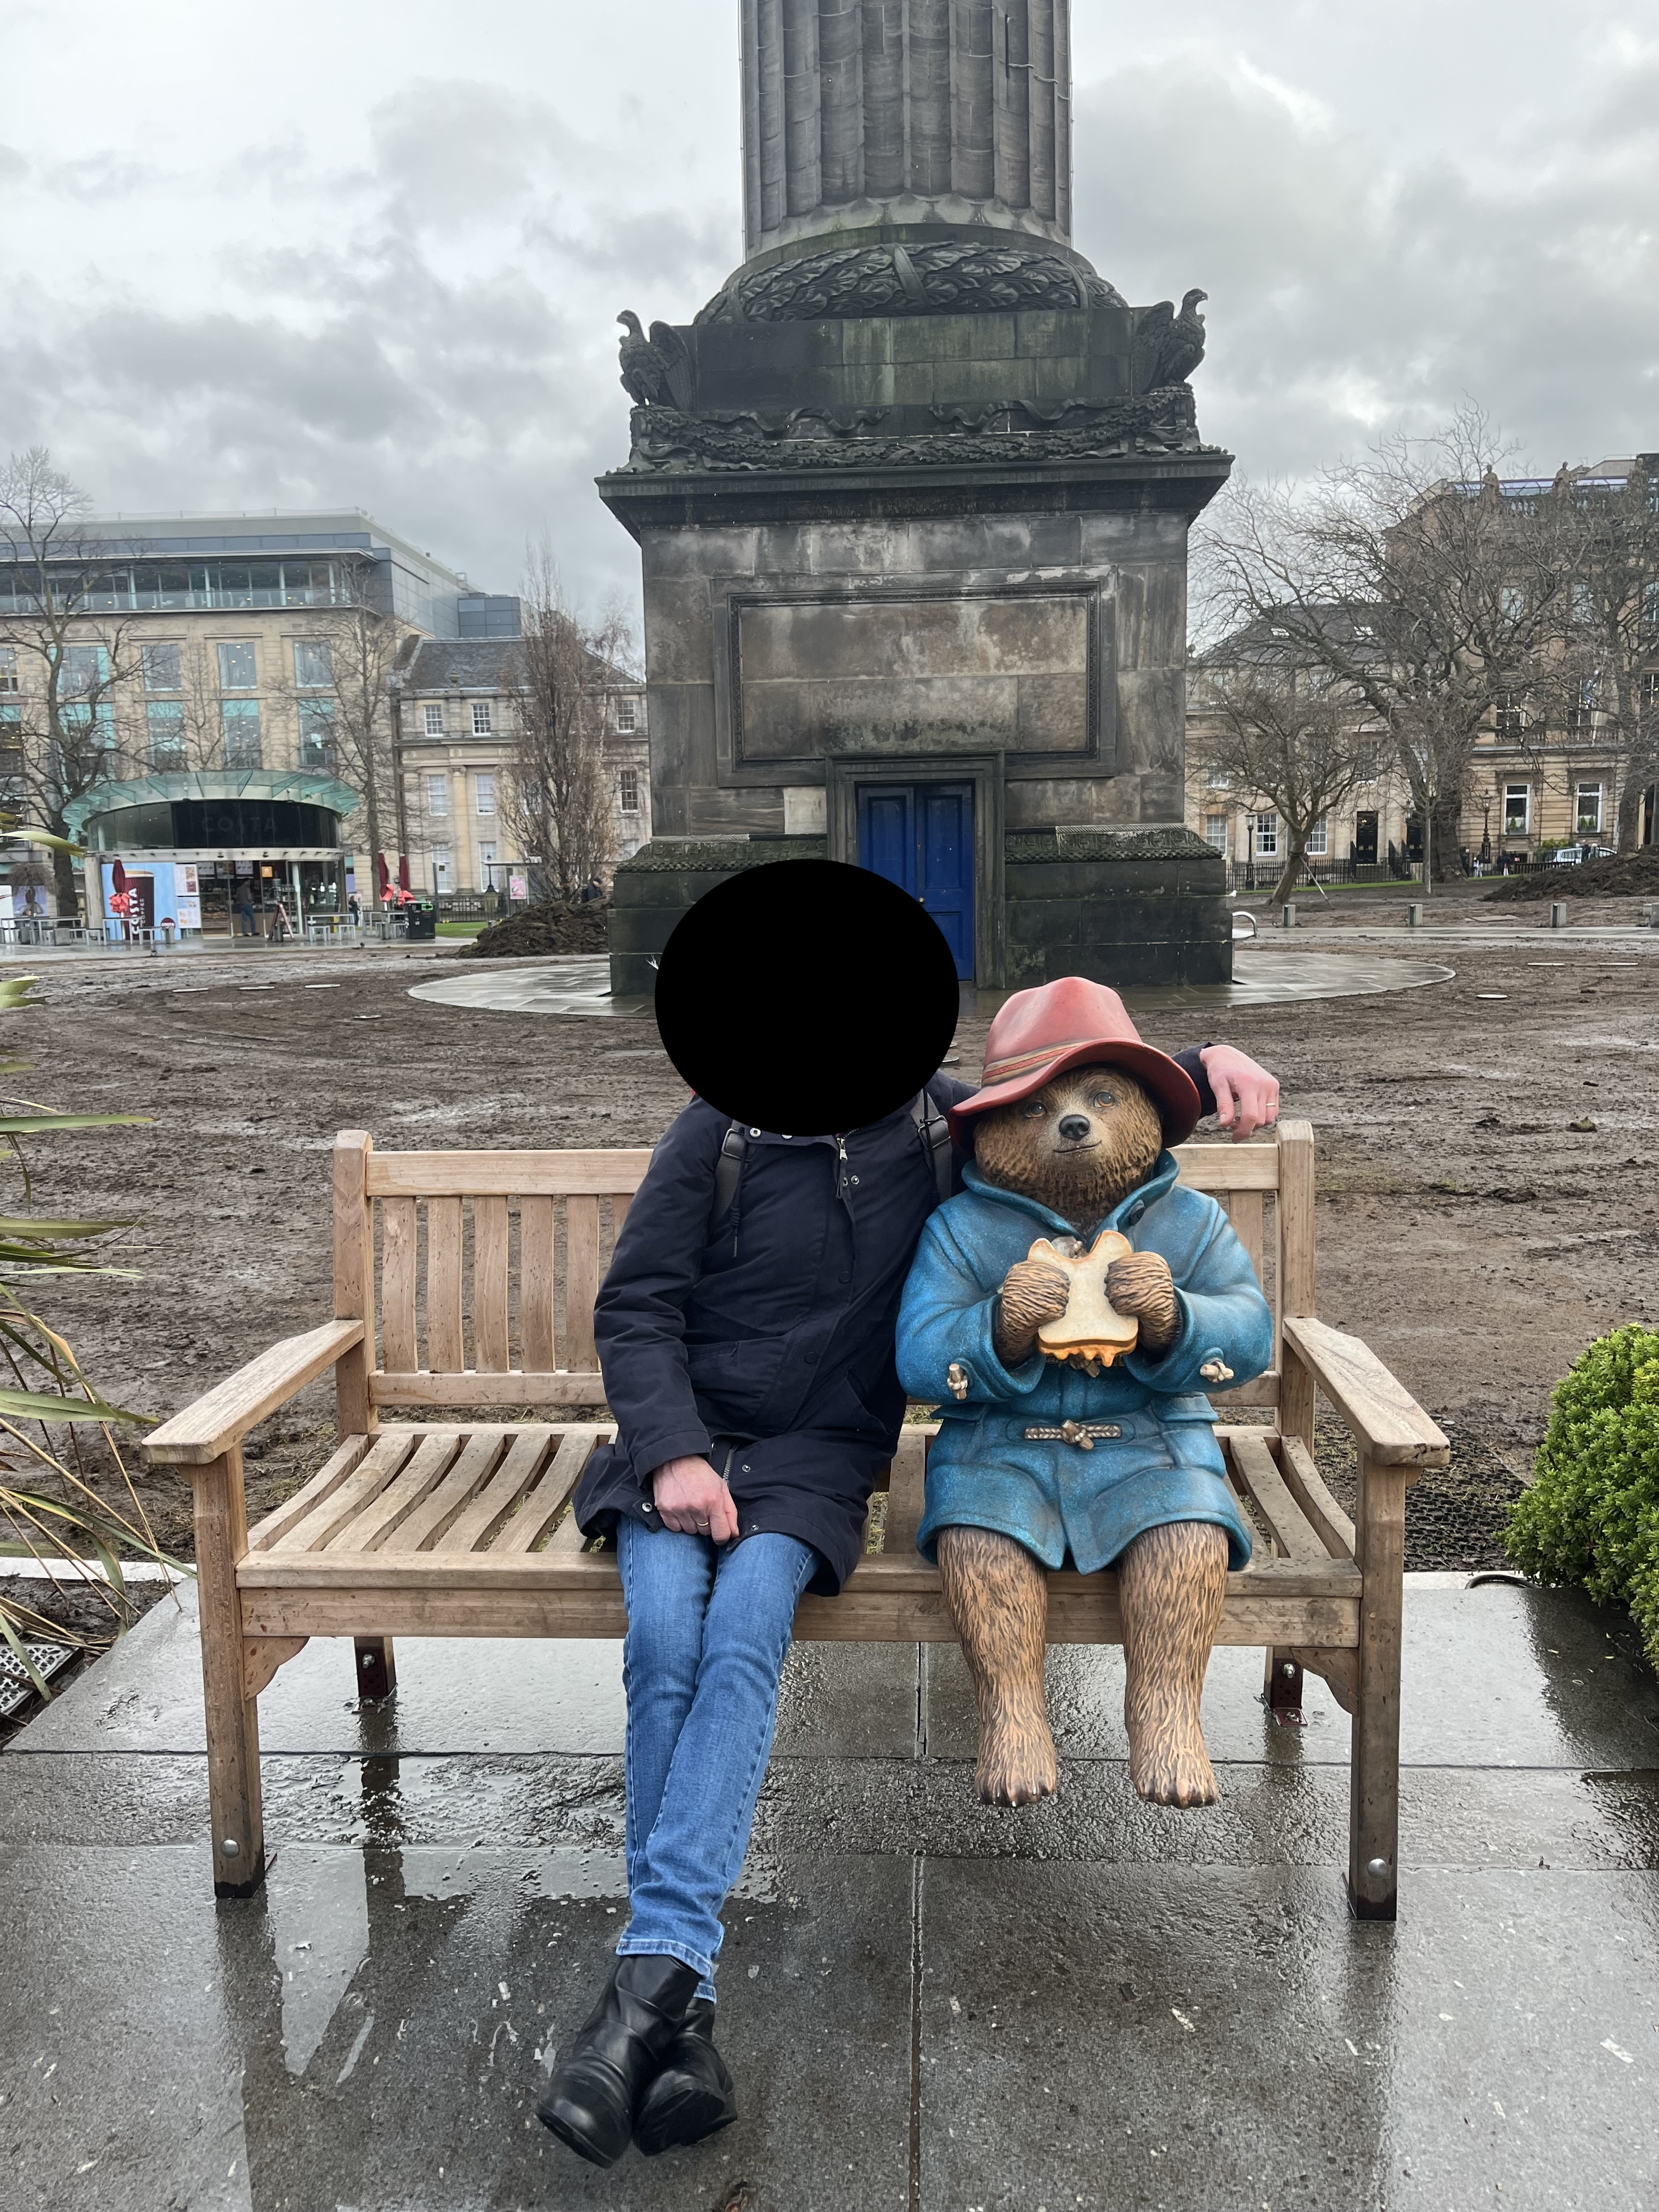
\includegraphics[width=1\linewidth]{img/paddington.jpg}
%     \caption{Paddington Bear in front of Melville Monument}
%     \label{fig:paddington}
% \end{figure}

\begin{figure}
    \centering
    \includegraphics[width=1\linewidth]{img/map_numbered.png}
    \caption{Map of St Andrews Square (Source OpenStreetMaps.org), position of the plaques are \textbf{1.} Original \textbf{2}. Updated \textbf{3}. Stevenson \textbf{4.}(\textbf{a} and \textbf{b}) Temporary}
    \label{fig:st_andrews_map}
\end{figure}

\begin{figure}
    \centering
    \includegraphics[width=1\linewidth]{img/melville_graffiti.jpg}
    \caption{Graffiti on Melville Monument: Source \cite{daily_2020}}
    \label{fig:dundas_graffiti}
\end{figure}
\begin{figure}
    \centering
    \includegraphics[width=1\linewidth]{img/robert_dundas_defaced.jpg}
    \caption{Graffiti on Robert Dundas Memorial. Source \cite{hay_2020_3}}
    \label{fig:robert_graffiti}
\end{figure}

\begin{figure}
    \centering
    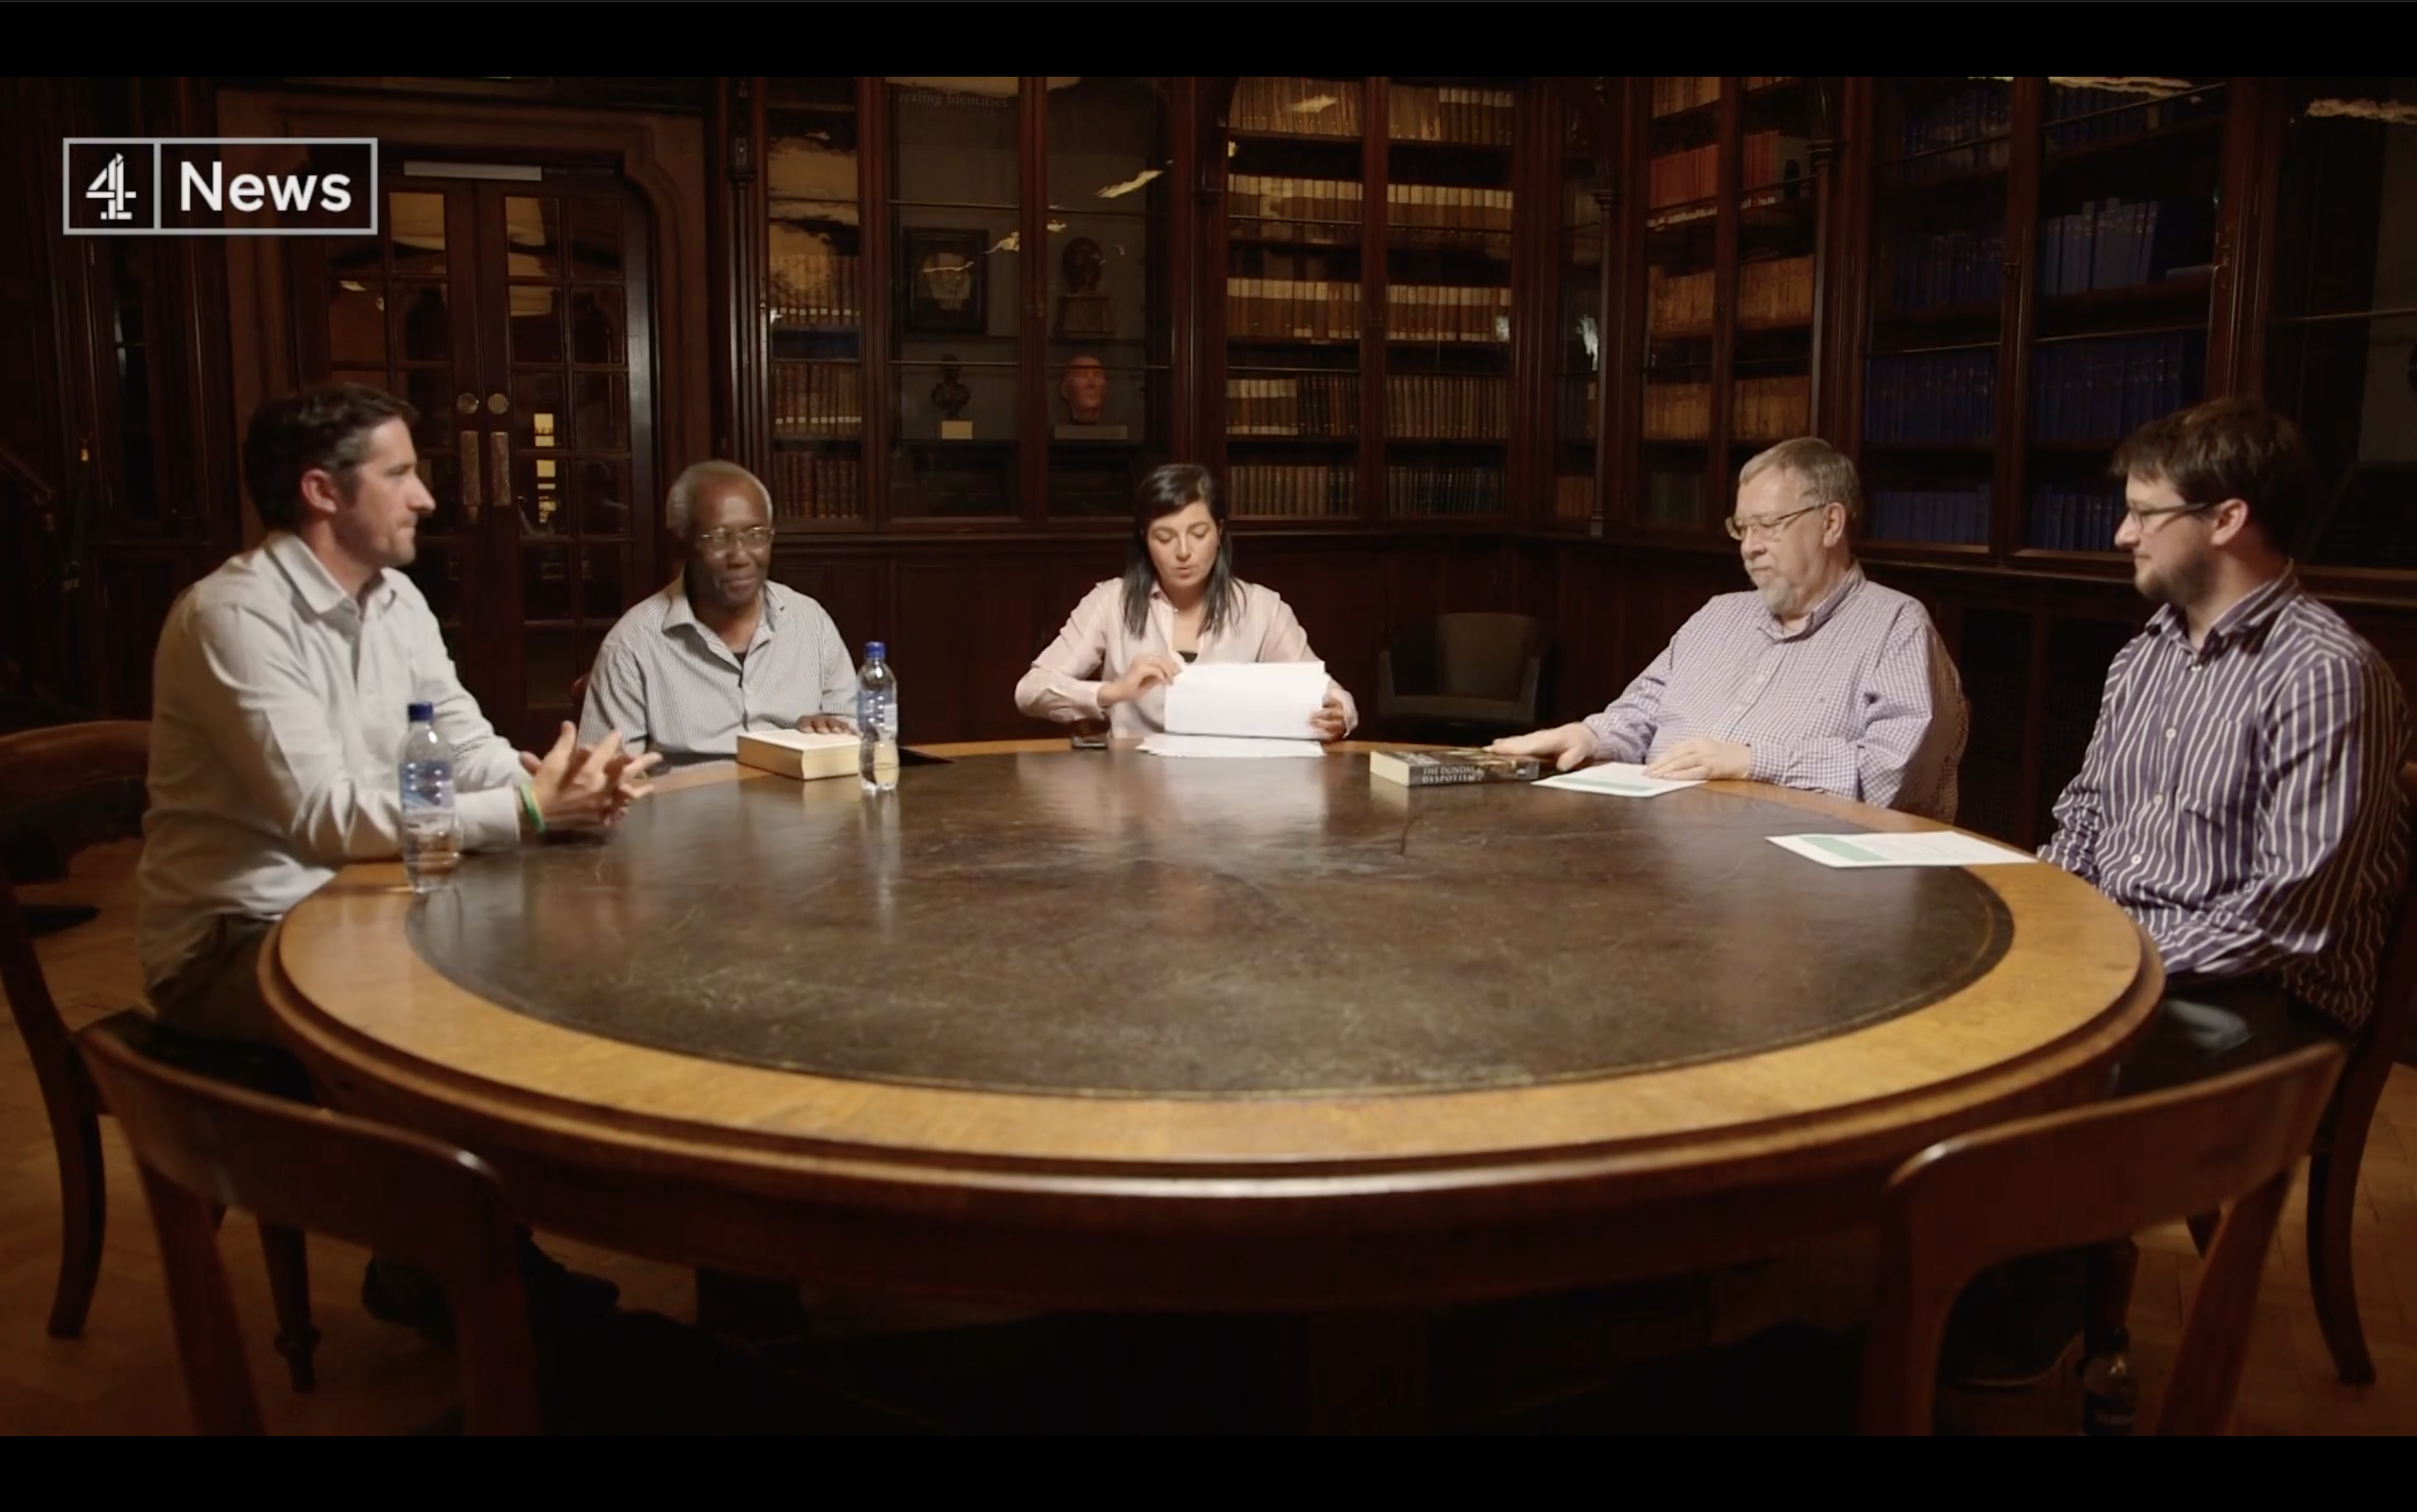
\includegraphics[width=1\linewidth]{img/plaque-committee-2.png}
    \caption{The ``plaque committee''. Source Channel 4 News 
    \cite{c4n_2018}. From left to right: Bobby Dundas, Geoff Palmer, Unknown, Michael Fry, Adam Ramsay}    
    \label{fig:plaque-committee}
\end{figure}

\begin{figure}
    \centering
    \includegraphics[width=1\linewidth]{img/ramsay-plaque.jpg}
    \caption{Plaque installed by Adam Ramsay 10 May 2016 \cite{ramsay_2016}}
    \label{fig:ramsay-plaque}
\end{figure}
\end{appendices}

\end{document}
